\chapter{Implementácia}\label{chap:implementacia}
Začiatkom tejto kapitoly v stručnosti opisujeme použité technológie a taktiež uvádzame dôvody, prečo sme si ich zvolili. 
Jednotlivé časti programu sme zhrnuli do viacerých súvislých celkov, ktoré sme podrobne charakterizovali a preskúmali. Najdôkladnejšie sa venujeme častiam programu, ktoré považujeme za zaujímavé, z dôvodov ich zložitosti alebo kvôli metóde, ktorú sme pri ich riešení použili. 

\section{Použité technológie}

\subsection{C++}
Jazyk C++ vznikol rozšírením jazyka C o triedy a iné rysy objektovo orientovaného programovania. Jedná sa o 
jeden z najznámejších a najobľúbenejších programovacích jazykov za posledných pár dekád. Vďaka jeho obľúbenosti bolo vytvorených mnoho interných ale aj externých knižníc a nadstávb, čo je jeden z dôvodov, prečo sme si ho zvolili na prácu. 

Vďaka tomu, že má tento jazyk nízkoúrovňové a zároveň aj vysokoúrovňové črty programovacích jazykov, umožňuje dobrý interface na efektívny manažment pamäťových a procesových zdrojov. Spomínaná vlastnosť jazyka je užitočná pri pamäťovo a výpočtovo náročných algoritmoch, s ktorými sa pri objemovej grafike zaručene stretneme.

\subsection{OpenGL}
V práci sme si ako prvé uvedomili nevyhnutnosť vizualizácie voxelového priestoru a na túto úlohu sme vybrali knižnicu OpenGL.

Jedná sa o jednu z najznámejších a najpoužívanejších open source multi-platformových API na interakciu s grafickými akcelerátormi (GPU). Dobre špecifikovaný OpenGL štandard má jazykové väzby na mnohé často používané programovacie jazyky \cite{OpenGL}.
Funkcie OpenGL API sú dobre definované a sú volateľné aj z jazyka C++, ktorý sme si zvolili ako hlavnú implementačnú technológiu. Táto knižnica vo všeobecnosti ponúka široké množstvo výhod, akou je napríklad veľké množstvo podrobných rád a návodov, ako s knižnicou narábať a zároveň má OpenGL veľmi podrobne spracovanú dokumentáciu. Aj toto bol jeden z dôvodov, prečo sme si ju zvolili pre náš účel.

%Aby sme vedeli efektívne využívať možnosti, ktoré nám OpenGL ponúka, je potrebné nahliadnuť trocha pod povrch tejto knižnice na renderovaciu pipeline.
%
%Ako možno vidieť na obrázku \ref{pipeline} ... strucny opis pipeline
%
%
%\begin{figure}[ht!]
%	\centering
%	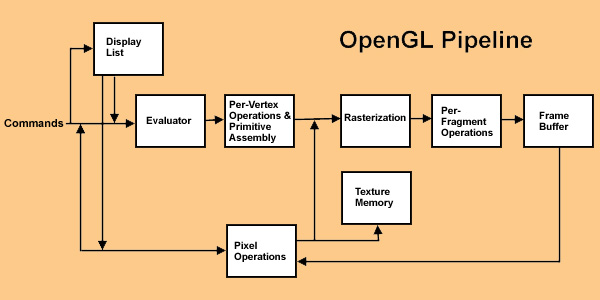
\includegraphics[width=90mm]{pipeline.JPG}
%	\caption{OpenGL pipeline}
%	\label{pipeline}
%\end{figure}

\subsection{DevIL}
Počas implementácie sa ukázalo, že je potrebné načítať bitmapy, ktoré sa následne použili ako textúry, alebo sa pretransformovali na jednovrstvový voxelový objekt. Ako prvá sa nám ponúkla knižnica \textit{DevIL} \cite{devil}, ktorú sme nakoniec aj v práci použili.

DevIL, pôvodne pomenovaná ako OpenIL, je programátorská knižnica, slúžiaca na načítavanie obrázkov širokej škály formátov do pamäti. Udržiava podobné menné konvencie ako OpenGL a veľmi dobre s ním aj spolupracuje.

\subsection{Microsoft Visual Studio 2012}
Spoločnosť \textit{Microsoft} ponúka vysokokvalitné vývojové prostredie \textit{Microsoft Visual Studio} \cite{mvs}, ktoré je pre študentov našej fakulty dostupné zdarma a voľne použiteľné na nekomerčné účely.
Jeho integrovanou súčasťou je aj prostredie na vytváranie GUI pre Win32, čo je jeho hlavná výhoda, ktorú sme zohladňovali pri výbere toho správneho IDE.
V prvých fázach práce sme volili verziu 2010 Express, ktorá však neobsahovala možnosť lepšieho syntax highlightu, čo bolo pri rozsiahlosti kódu pomerne dôležité, a tak sme nakoniec prešli na verziu 2012, ktorá nám plne vyhovovala.

\subsection{Assimp}
Na loadovanie povrchových modelov za účelom voxelizácie sme vybrali knižnicu \textit{Assimp} \cite{assimp}, ktorá je taktiež voľne dostupná.

Jej hlavnými výhodami sú, že poskytuje pre a post-processing, má jednoduchý interface a podporuje tucty rôznych 3D súborových formátov.

Nevýhodami naopak sú, že má komplikovanejšiu inštaláciu, niektoré zdokumentované triedy nie sú správne implementované alebo nie su implementované vôbec a to často spôsobuje problémy, ktoré sa môžu objaviť pri práci.
\subsection{pugixml}
Na export a import dát z celej scény sme sa rozhodli použiť jazyk XML a nami navrhnutú podrobnú štruktúru opisujeme nižšie v tejto kapitole. Keďže parsovanie takýchto štruktúr nie je úplne triviálne a je vytvorených už mnoho existujúcich riešení, využili sme túto možnosť a siahli po knižnici \textit{pugixml} \cite{pugixml} na parsovanie XML súborov.

Dôvodom prečo sme si ju zvolili je, že sa jedná o extrémne rýchlu knižnicu, ktorá vytvorí DOM strom z XML súboru, takže zaručuje jednoduché použitie.

\section{Rendering}
Na rendering sme použili spomínanú knžinicu OpenGL s jej programovým rozšírením OpenGL Utility Toolkit (GLUT) \cite{glut}.
\subsection{Rendering voxelu}
Predpokladáme, že voxel ako základný element voxelového priestoru sa bude v scéne nachádzať v pomerne veľkých objemoch. Z tohoto dôvodu bolo potrebné nájsť spôsob, ako jeden voxel čo najúspornejšie vyrenderovať.
Na tento účel sme sa rozhodli použiť display listy. Display list je séria príkazov OpenGL, ktoré sú skompilované a uložené, spolu s inými dátami o objekte na GPU \cite{DisplayList}.
Vďaka tomu používanie displaylistov redukuje komunikáciu medzi GPU a CPU, ktorá je v procese renderovania časovo náročná. Display listy sú teda vhodné na rendering objektov s rovnakou topológiou, ktoré sa v scéne vyskytujú veľmi často. Keďže každý voxel je objekt v tvare kocky s rôznymi vlasnosťami akou je napríklad farba, môžme použiť jedinú zabudovanú funkciu GLUTu: 
\begin{verbatim}
   void glutSolidCube(GLdouble size)
\end{verbatim}
alebo tiež:
\begin{verbatim}
   void glutWireCube(GLdouble size)
\end{verbatim}
Spôsob renderovania voxelu ešte ovplyvňujú jeho vnútorné vlastnosi ako farba, flag určujúci označenie voxelu, a taktiež nastavenie renderingu ako napríklad shading, backface culling, zobrazenie wireframu alebo tiež veľkosť vzorky.
\subsection{Rendering objektu}
Ako sme spomenuli o sekciu vyššie, bolo potrebné nájsť spôsob ako čo najviac ušetriť renderovací proces. Takéto vylepšenie je možné spraviť aj pri renderingu objektov, pretože veľké množstvo voxelov býva prekrytých inými. Použili sme preto veľmi jednoduchú, ale účinnú metódu, ktorá rozhoduje, či voxel zobraziť, podľa toho, io je ohraničený zo všetkých šiestich strán alebo nie je. Takto sme sa zbavili vykreslovania všetkých voxelov, ktoré nebolo možné nikdy vidieť.
\subsection{Rendering scény}
Scéna sa skladá z viacerých voxelových objektov, ktoré je potrebné pri zobrazovaní posunúť správnou translačnou maticou na svoju pozíciu. Plávajúce objekty v priestore môžu na užívateľa programu pôsobiť dezorientujúco, a preto sme pridali do scény dva vizuálne elementy a tými sú podlaha a začiatok karteziánskej sústavy s troma osami. 


\section{Voxelové Objekty}\label{voxelObjects}
Sekundárny element v našom priestore po voxeloch je voxelový objekt, ktorý o sebe uchováva sadu základných informácií, z ktorých najdôležitejšie sú pozícia, dané rozmery a voxely, ktoré mu prislúchajú.

Každý objekt v scéne predstavuje samostatný ohraničený voxelový priestor. Na jeho reprezentáciu sme sa rozhodli použiť trojrozmerné pole, ktorého výhodou je priamy prístup k voxelom prostredníctvom ich indexov.
Vďaka tejto vlastnosti je možné rýchlo a jednoducho procedurálne generovať voxelové objekty a ich rôzne transformácie.

\subsection{Základné tvary}
Pre jednoduchšie a rýchlejšie modelovanie väčšina 3D grafických nástrojov ponúka sadu základných telies, ktoré sú pri práci často využívané. Takýmto postupom sme sa inšporovali i my a zhotovili sme sadu objektov\footnote{Kôli diskrétnosti voxelového priestoru, spomenuté objekty predstavujú iba aproximáciu konkrétnych geometrických útvarov.}, ktoré sa generujú na základe jednoduchej matematiky. Takéto generovanie by sme mohli zovšeobecniť na nasledujúci algoritmus:


\begin{algorithmic}
	\For{$(i,j,k) = (0,0,0) \to (width, height, depth)$}
		\If{ $v\_telese(i,j,k)$ } // funkcia je špecifická pre každý útvar
			\State Pridaj voxel do $Objekt$u na pozíciu (i,j,k)
		\Else
			\State Pridaj $NULL$ do $Objekt$u na pozíciu (i,j,k)
		\EndIf
	\EndFor
\end{algorithmic} 

	\subsubsection{Kváder}
	Vytvorenie kvádra je veľmi jednoduché. Jeho podmienka v spomenutom algoritme je funkcia vracajúca vždy hodnotu \textit{TRUE}. Takúto funkciu môžme odstrániť a v jednoduchosti môžme povedať, že objekt inicializovaný na dané rozmery iba naplníme voxelmi príslušnej farby.
	\subsubsection{Elipsoid}
	Elipsoid je povrchové teleso dané rovnicou:
	\begin{displaymath}
	\frac{x^2}{a^2} + \frac{y^2}{b^2}+ \frac{z^2}{c^2} = 1 
	\end{displaymath}
	Keďže v našom prípade budeme potrebovať elipsoid so stredom v bode \\ \begin{math}S = (s_1,s_2,s_3)\end{math}
	k úžitku nám bude všeobecnejšia rovnica:
	\begin{displaymath}
		\frac{(x - s_1)^2}{a^2} + \frac{(y - s_2)^2}{b^2}+ \frac{(z - s_3)^2}{c^2} = 1 
	\end{displaymath}
	Kde \textit{a}, \textit{b}, \textit{c} určujú dĺžky poloosí v smere osí \textit{x}, \textit{y}, \textit{z} ako možno vidieť na obrázku \ref{elipsoid}.
	
	Vďaka tejto rovnici môžme ľahko určiť, ktoré body sa nachádzajú v telese alebo mimo telesa, vytvorením nerovnice, ktorá vznikne nahradením znamienka = za \begin{math} < \end{math} alebo \begin{math} > \end{math}.

	\begin{figure}[ht!]
	\centering
	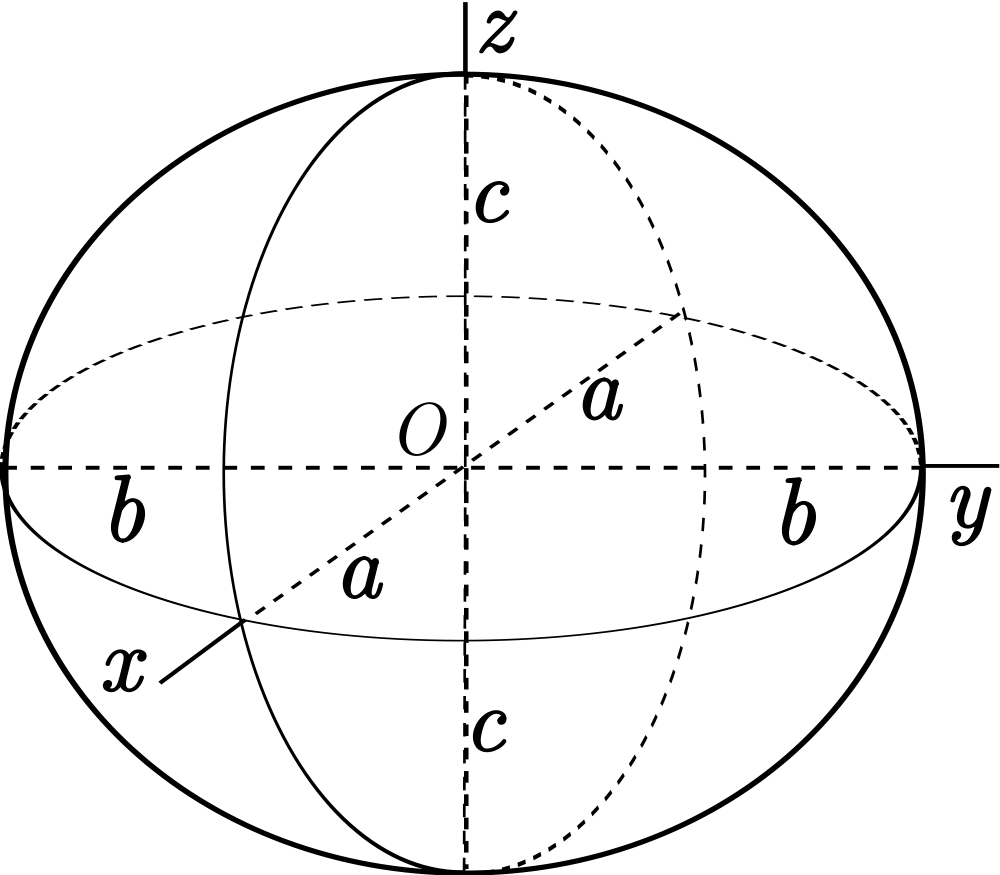
\includegraphics[width=90mm]{ellipsoid.png}
	\caption{Elipsoid}
	\label{elipsoid}
	\end{figure}
	
	V našom prípade sú hodnoty \textit{a}, \textit{b}, \textit{c} nahradené za \textit{width/2}, \textit{height/2}, \textit{depth/2}, hodnoty \textit{x}, \textit{y}, \textit{z} za \textit{i}, \textit{j}, \textit{k} a stred S = (width/2, height/2, depth/2). Naša funkcia rozhodujúca, či sa voxel nachádza v telese by mohla vyzerať takto:
	\begin{displaymath}
		\frac{(i - (width/2))^2}{(width/2)^2} + \frac{(j-(height/2))^2}{(height/2)^2}+ \frac{(k - (depth/2)) ^2}{(depth/2)^2} < 1 
	\end{displaymath}
	zjednodušene:
	\begin{displaymath}
			\frac{(i - s_1)^2}{s_1^2} + \frac{(j-s_2)^2}{s_2^2}+ \frac{(k - s_3) ^2}{s_3^2} < 1 
	\end{displaymath}
	a ešte jednoduchšie:
	\begin{displaymath}
		(\bar{p})^2 < 1 \textrm{, kde }
		\bar{p} = (\frac{i - s_1}{s_1}, \frac{j - s_2}{s_2}, \frac{k - s_3}{s_3}) 
	\end{displaymath}
	\subsubsection{Valec}
	Základ na vygenerovanie valca je podobný ako pre elipsoid, s tým rozdielom, že potrebujeme rovnicu posunutej elipsy do stredu \begin{math}S = (s_1, s_2)\end{math} :
	\begin{displaymath}
		\frac{(x - s_1)^2}{a^2} + \frac{(y - s_2)^2}{b^2} = 1 
	\end{displaymath}
	Pre každú vrstvu objektu v našom prípade v smere osi \textit{y} (zanedbávame teda y-ovú súradnicu respektíve súradnicu j) zisťujeme, či sa bod nachádza v elipse alebo mimo nej. Táto elipsa je určená stredom \begin{math}S = (wdith/2, depth/2)\end{math} a rovnakými rozmermi, teda \begin{math}a = wdith/2, b = height/2\end{math}. Výsledná nerovnica vyzerá nasledovne:
	\begin{displaymath}
		\frac{(i - (width/2))^2}{(width/2)^2} + \frac{(k - (depth/2)) ^2}{(depth/2)^2} < 1  
	\end{displaymath}
	Toto môžme zjednodušiť rovnako ako v predchádzajúcom prípade na:
	\begin{displaymath}
		(\bar{p})^2 < 1 \textrm{, kde }
		\bar{p} = (\frac{i - s_1}{s_1},\frac{k - s_3}{s_3})
	\end{displaymath}	
	\subsubsection{Ihlan}
	Pre pochopenie základného konceptu tvorby diskrétneho ihlanu, môžme problém zjednodušiť na vygenerovanie diskrétneho rovnoramenného trojuholníka.
	Počet bodov pre prvý a posledný riadok takéhoto trojuholníka vieme ľahko zistiť. Prvý riadok obsahuje 1 alebo 2 body podľa toho, či je šírka trojuholníka párna alebo nepárna, no a posledný riadok obsahuje počet bodov rovný šírke trojuholníka. Aby sme získali počet bodov, ktoré sa nachádzajú v riadkoch medzi prvým a posledným, stačí nám použiť lineárnu interpoláciu bodov: 
	$X = (x,y), A = (x_0, y_0), B = (x_1, y_1)$ 
	\begin{displaymath}
	\frac{y - y_0}{x - x_0} = \frac{y_1 - y_0}{x_1 - x_0} 
	\end{displaymath}
	Pre nás je x hľadaný počet bodov na riadok $j$, y je spomenutý riadok $j$, $A = (f , 1)$, kde $f$ je 1 alebo 2 a $B = (width, height)$. Z toho nám vyplýva:
	\begin{displaymath}
		x = \frac{(j - 1) . (width - f)}{height - 1} + f
	\end{displaymath}
	Teraz nám už stačí umiestniť body na stred dvojrozmernej mapy, čo je pomerne jednoduché.
	Túto myšlienku pre diskrétny trojuholník už ľahko rozšírime do priestoru.
	\subsubsection{Kužeľ}
	Kužeľ je najkomplikovanejším tvarom, z pomedzi všetkých spomínaných. Avšak nie je potrebné vymýšlať nijaký nový spôsob na jeho vytvorenie, keďže tento tvar získame kombináciou už dvoch vyššie spomenutých metód. Vďaka metódam pre valec a pre ihlan môžme získať veľmi pekný voxelový kužeľ.


\subsection{Booleanovské operácie nad objektami}
Známa modelovacia paradigma CSG využíva na vytvorenie výsledného modelu booleanovské operácie. Potrebnosť tohoto prvku vo voxelovom editore sme si uvedomili aj my, a tak sme sa rozhodli implementovať základné operácie akými sú \textit{AND}, \textit{OR}, \textit{NOT} a \textit{XOR}.
Vo všobecnosti by sa dal algoritmus, ktorý sme vytvorili, pre vstupné objekty \textit{A} ,\textit{B} a výstupný \textit{C} opísať v troch krokoch:
\begin{enumerate}
\item Získanie bounding boxu pre C.
\item Zistenie pozície nového objektu C.
\item Postupné vkladanie voxelov do objektu C z objektov A,B na základe danej logickej funkcie.
\end{enumerate} 

\subsection{Transformácie objektov}
\subsubsection{Translácia}
Jedná sa o základnú transformačnú funkciu objektov, ktorej úlohou je zmeniť polohu objektu v scéne. Vyznačuje sa jednoduchou implementáciou, keďže nie je potrebné nijakým spôsobom meniť štruktúru voxelov v objekte.
V časti \ref{tools} \textit{Nástroje} v podsekcii \ref{moveTool} \textit{Posun objektov} je bližšie špecifikované ako môže užívateľ danú funkcionalitu používať.

\subsubsection{Škálovanie}
Problém vzniku dier pri škálovaní sa z 2D rasterového priestoru prenáša aj do 3D voxelového priestoru. Na jeho riešenie sme použili algoritmus \textit{Nearest-neighbor interpolation}, ktorý je veľmi jednoduchý, no napriek tomu dosahuje primerané výsledky.

Škálovať voxelový objekt je možné vo všetkých troch rozmeroch súčasne zadaním škálovacieho faktoru pre každý smer osi zvlášť.
\subsubsection{Rotácia}
Pri rotácii podobne ako pri škálovaní hrozí pri určitých hodnotách vznik dier. Tento problém sme riešili prepracovaním algoritmu na rotáciu bitmapy opísanom v článku od Michela Leunena \cite{Rotate}. 

Základnou myšlienkou je zistenie nových rozmerov obrázka a v našom prípade objektu pomocou danej rotačnej matice v priestore. Následne už len prechádzame všetkými bodmi nového objektu a snažíme sa získať voxely, pomocou spomenutej matice, z pôvodného nezrotovaného objektu. Takýmto spôsobom sme dosiahli pomerne uspokojivé výsledky.

\subsubsection{Mapovanie textúr}
Kôli jednoduchosti sme zvolili planárne mapovanie textúr na objekt podľa osí. Teda je možné namapovať textúru z celkovo 6 rôznych strán (2 pre každú os). Algoritmus mapovania textúry spočíva v štyroch krokoch:
\begin{enumerate}
\item Naškálovanie obrázka na potrebnú veľkosť. Toto zabezpečí knižnica DevIL.
\item Napasovanie obrázka na danú stenu objektu.
\item Vyslanie lúča z každého bodu obrázka smerom na objekt. \\ 
\begin{small}(Takto získame potrebný voxel.)\end{small}
\item Každý získaný voxel zafarbíme príslušnou farbou pixelu.
\end{enumerate}

\section{Nástroje}\label{tools}
Akýkoľvek editor, ktorý si predstavíte, nemôže existovať bez editačných nástrojov. V tejto časti opíšeme, aké nástroje náš voxelový editor ponúka, ich stručný opis a v prípade zaujímavých nástrojov podrobnejší opis ich implementácie.

Správu nástrojov sme riešili podľa nasledujúceho UML diagramu \ref{uml}.

\begin{figure}[ht!]
	\centering
	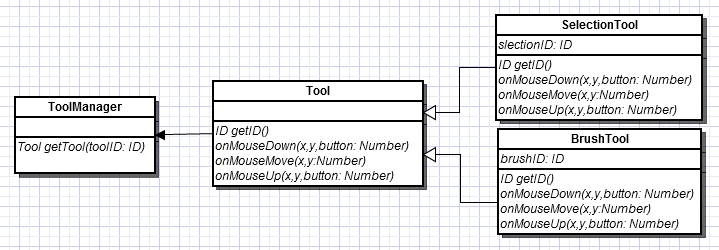
\includegraphics[width=0.9\textwidth]{tool.jpg}
	\caption{Triedny diagram pre nástroje}
	\label{uml}
\end{figure}


Základom je abstraktná trieda Tool, ktorá obsahuje virtuálne metódy:
\begin{verbatim}
   void mouseDown(int x, int y, int button)
   void mouseMove(int x, int y)
   void mouseUp(int x, int y, int button)
   ID getID()
\end{verbatim}
Hlavnou spravujúcou triedou je ToolManager, ktorý uchováva všetky objekty odvodené od triedy Tool. Vďaka spôsobu akým je manažment nástrojov navrhnutý, môžeme rôzne typy nástrojov získavať jednoducho z ToolManagera iba vďaka konkrétnemu ID.

\subsection{Selekcia}
Tento nástroj má dve funkcionality. Prvou je selekcia objektov a druhou selekcia voxelov na udalosť kliknutia na daný objekt.
\subsubsection{Selekcia objektov}
Označovanie objektov prebieha tak, že sa z miesta obrazovky vyšle lúč a následne sa zistia priesečníky so všetkými objektami v scéne. Takto získame pole objektov, z ktorých vyberieme objekt najbližší ku začiatočnému bodu lúča. Keďže predpokladáme, že voxelových objektov nebude v scéne príliš veľa, táto metóda je pre nás dostačujúca.
\subsubsection{Selekcia voxelov}
Od selekcie voxelov na kliknutie očakávame okamžitú spätnú väzbu. Ak by sme použili rovnakú metódu, ako na objekty, museli by sme zisťovať priesečníky s obrovským množstvom elementov, čo by spôsobovalo značné oneskorenie. Preto sme sa rozhodli využiť fakt, že každý voxelový objekt je umiestnený v pravidelnej trojrozmernej mriežke.

V prvej fáze zisťujeme miesto vniknutia lúču do objektu.
Na tomto mieste získame pozíciu bunky, kde by sa mohol nachádzať voxel.
Ak sa na danej pozícii žiaden voxel nenachádza, zistíme miesto, v ktorom lúč z bunky vychádza.
Podľa tohoto miesta zistíme susediacu bunku, do ktorej lúč vošiel.
Ak sa ani v nej voxel nenachádza postupujeme ďalej v cykle, kým nenarazíme na nenullový voxel alebo lúč nevylezie z objektu von. \\

\begin{minipage}{0.9\textwidth}
Opísaný algoritmus vyzerá asi takto:

\begin{algorithmic}
	\Function{getVoxel}{$Luc, Objekt$}
		\State $Priesecnik \gets $ Vypočítaj priesečník $Luc$a a $Objekt$u
		\State $Pozicia \gets $ Získaj pozíciu bunky v mieste $Priesecnik$
		\While{$Pozicia$ sa nachádza v $Objekt$e} 
			\State $Voxel \gets $ Voxel na pozícii $Pozicia$ v $Objekt$e 
			\If{$Voxel \neq NULL$} 
				\State \Return $Voxel$
			\EndIf 
			\State $Pozicia \gets$ Získaj susednú pozíciu bunky, kam sa dostal $Luc$ 
		\EndWhile
	\EndFunction \\
\end{algorithmic} 
\end{minipage}
\eject

Na obrázku \ref{invader} je zobrazené fungovanie algoritmu. 

\begin{figure}[!h]
	\centering
	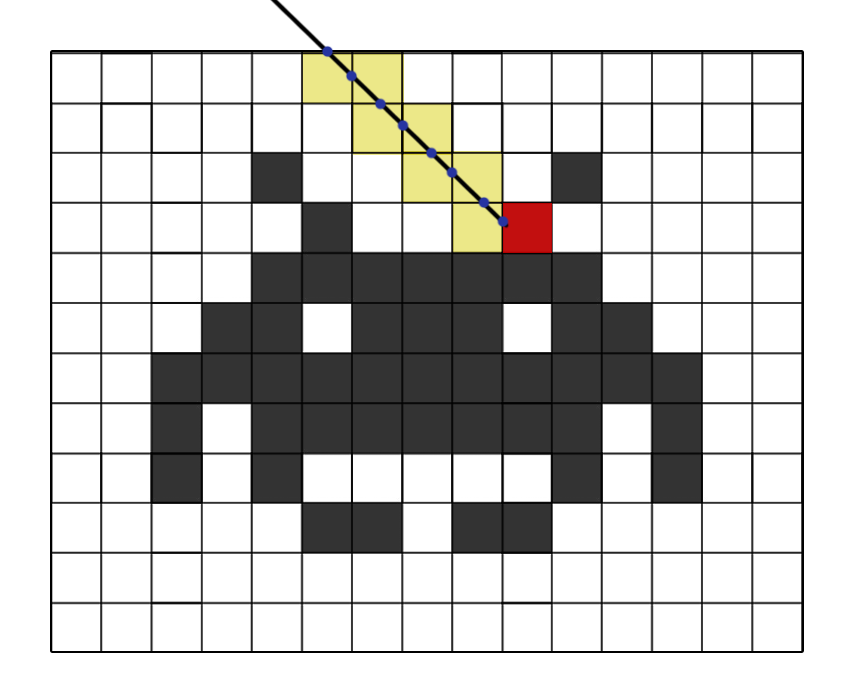
\includegraphics[width=90mm]{getVoxel.png}
	\caption{Vizualizácia fungovania algoritmu getVoxel}
	\label{invader}
\end{figure} 



\subsection{Štetec}
	Taktiež aj tento nástroj poskytuje dve funkcionality. Tou prvou je pridávanie voxelov na povrch objektu a tou druhou je zafarbovanie zakliknutých voxelov.
	Základom tohoto nástroja, ako aj mnohých nasledujúcich je opísaná funkcia na získavanie voxelov.
	Pri pridávaní voxelu sa získa kliknutý voxel a naň sa prilepí ďalší, zafarbený na natavenú farbu štetca. Pri zafarbovaní sa jednoducho zakliknutý voxel prefarbí podľa farby štetca. 
\subsection{Guma}
	Tento nástroj využíva funckiu získavania voxelov na ich mazanie. Pri zmazaní voxelu sa lokálne upravia okolité voxely, tak aby boli viditeľné. Teda sa im nastaví flag \textit{visible} na \textit{TRUE}.
\subsection{Kvapátko}
	Kvapátko je nástroj, ktorý už celé desaťročia mätie užívateľov svojím názvom. Slúži na získavanie farby z voxelu na kliknutie, preto bola aj pre tento nástroj potrebná funkcia na získavanie voxelu. 
\subsection{Výplň}
	Posledným nástrojom z rady implementovaných, ktorý používaja funkciu získavania voxelu pomocou lúča, je výplň. Tento nástroj zafarbí všetky voxely objektu, ktoré sú tranzitívne spojené so zakliknutým voxelom a zafarbí ich na farbu nastavenú v prostredí. To, že sú dva voxely spojené chápeme tak, že sú k sebe priamo susediace a zároveň sú rovnakej farby. Opísana procedúra priamo zachytáva algoritmus \textit{flood fill}, ktorý je len potrebné preniesť do priestoru.
\subsubsection{3D flood fill} 
	S veľmi pochabými úmyslami sme sa pustili do implementácie algoritmu rovno dvoma spôsobmi. \\
	Ako prvé sme zvolili rekurzívne riešenie a algoritmus prehľadávania do hĺbky. Funkciu bolo jednoduché implementovať, avšak už pri prvom testovaní sme narazili na veľký problém. Neuvedomili sme si, že pri veľkom počte voxelov sa funkcia vnára príliš hlboko do seba a teda nevyhnutne spôsobuje chybu pretečenia zásobníka
	
	Nefungujúcu funkciu bolo následne nutné prepísať tak, aby neobsahovala rekurziu. Tento problém sme vyriešili použitím radu a teda sme nahradili prehľadávanie do hĺbky, algoritmom prehľadávania do šírky.
	Naše riešenie teda vyzerá asi takto:
	
	\eject
	
	\begin{algorithmic}
		\Function{flood\_fill3D}{$indeces$}  
			\State $Visited \gets$ [ ]
			\State $Queue \gets [indeces]$
			\Repeat  
				\State $position \gets$ pop positon from $Queue$
				\If {$\NOT$($position$ in $Visited)$}
					\State Change color of voxel at $position$
					\ForAll{$position$ neighbours of same color}
						\State $Queue \gets Queue + [neighbour]$
					\EndFor
				\EndIf 
			\Until{$Queue$ is empty}
		\EndFunction \\
	\end{algorithmic} 
	
	{Finálne riešenie bolo ešte nutné pre urýchlenie upraviť tak, aby sme sa vyhli častému volaniu kopírovacích konštruktorov, použitím smerníkov.}
\subsection{Kamera}
	Tento nástroj je veľmi dôležitý pre užívateľa, aby sa rozumným spôsobom mohol orientovať v scéne. Ohnisko kamery je defaultne nastavené na stred celej scény, teda na bod $(0,0,0)$. Pri selekcii objektu pravým tlačidlom myši sa však ohnisko kamery zmení na stred označeného objektu.
	Kamera nám umožňuje orientáciu v scéne dvoma spôsobmi. Prvým je rotácia kamery okolo ohniska a druhým je približovanie sa alebo odďaľovanie od objektu, inak povedané zoom.
\subsection{Posun objektov}\label{moveTool}
	Označené objekty je možné posúvať na dragovaciu udalosť v troch rovinách. \\
	Kliknutie na objekt určí rovinu, v ktorej je možné objekt pohybovať podľa toho, na ktorú stenu užívateľ klikol. Okolo objektu sa následne zobrazí obdĺžnik, ktorý túto rovinu vizualizuje ako pomôcku pre užívateľa. Takéto riešenie je asi jediné svojho druhu, no napriek tomu ho považujeme za celkom jednoduché a intuitívne.


\section{Import/Export}\label{sec:io}
Modelovacie aplikácie akou je aj tá naša si vyžadujú import a export dát do a z programu. Rozhodli sme nájsť špecifikácie rôznych formátov voxelových súborov, ktoré už existujú, aby sme dosiahli čo najlepšiu variabilitu programu pri použití v praxi. Okrem ukladania dát do binárnych voxelových súborov je možné scénu exportovať do XML štruktúry alebo aj ako povrchový model vygenerovaný z voxelového.
\subsection{Polygónový model}
\subsubsection{Import}
Keďže všetky modely, ktoré sa nachádzajú v programe je možné uchovávať a zobrazovať iba v podobe voxelových objektov, import klasického povrchového modelu predstavuje nutnosť konverzie 3D meshu na voxely. Tento proces je tiež nazývaný \textit{voxelizácia}.
\eject
\subsubsection{Voxelizácia}
Vo všeobecnosti proces voxelizácie produkuje množinu hodnôt v pravidelnej trojrozmernej mriežke z objektov určených povrchovou reprezentáciou. Cieľom voxelizácie je vytvoriť voxelový objekt, ktorý je čo najbližšou možnou aproximáciou k originálnemu objektu. \cite{Voxelization}
Presnosť výsledku samozrejme závisí aj od rozmerov mriežky, ktoré si zvolíme. Kritickými miestami tohoto procesu môžu byť objekty s nulovou hrúbkou, alebo objekty s nekonvexnými dierami.

Riešenia opísané Georgom Passalisom \cite{Voxelization} využívajú možnosti GPU prostredníctvom funkcií OpenGL. Základná myšlienka spočíva v použití z-bufferov, vyprodukovaných povrchovými objektami, na voxelizáciu.
Algoritmus, ktorý prezentuje Karabassi potrebuje 3 páry z-bufferov, kde každá dvojica je určená pre jednu os. Kamera sa umiestni na všetkých 6 plôch pomyselného bounding boxu voxelizovaného objektu a s použitím ortogonálnej projekcie sa zapíšu dáta do bufferov. \cite{BufferVox}

Toto riešenie je pomerne jednoduché, avšak v istých prípadoch produkuje neželané výsledky. Ďalšia implementácia voxelizácie spomenutá v tomto článku rieši nedostatky tohoto algoritmu použítím komplikovaných shaderov, a preto sme sa rozhodli túto metódu nepoužiť a zvolili sme priamočiarejší prístup k problému.

Naše riešenie napasuje voxelizovaný objekt do mriežky s danými rozmermi a pre každú bunku mriežky určí, či sa jej stred nachádza v objekte alebo nie. Ak sa daný bod v objekte nachádza, pridáme voxel do objektu, ak sa nenachádza, tak nepridáme nič, respektíve pridáme nullovú hodnotu.
\eject
Približne takto vyzerá náš program: 

\begin{algorithmic}
	\State $\bullet$ Vytvor trojrozmernú mriežku \textit{M} s rozmermi $(width, height, depth)$
	\State $\bullet$ Naškáluj objekt \textit{O} do danej mriežky (tak aby sa objekt nedeformoval)
	\ForAll{$bunka \in M$}
		\If{ $bunka$ sa nachádza v $O$ }
			\State $\bullet$ Pridaj voxel do objektu.
		\Else
			\State $\bullet$ Pridaj $NULL$ do objektu.
		\EndIf
	\EndFor \\
\end{algorithmic} 

Takýto prístup je intuitívny a ľahko pochopiteľný aj pre laika. Rozhodujúcu úlohu v algoritme zohráva metóda zobrazená na obrázku \ref{ray}, ktorá determinuje, či sa bod nachádza v objekte alebo nie. Túto úlohu sme vyriešili tak, že sa z daného bodu vyšle lúč (polpriamka), a spočítajú sa priesečníky lúča s povrchom objektu. Ak ich počet je nepárny znamená to, že bod sa v objekte nachádza, inak sa v objekte nenachádza. Takto sa nám úloha posunula na ďalší podproblém zisťovania priesečníku polpriamky s polygónom. Keďže nájsť priesečník priamky s trojuholníkom je ľahšie ako s ľubovoľným polygónom, triangulizovali sme objekt už pri načítavaní zo súboru a potom sme mohli nájsť priesečník polpriamky s rovinou trojholníka a následne pomocou barycentrických súradníc sme rozhodli, či sa v ňom daný priesečník nachádza. 


Na obrázku \ref{ray} vidno fungovanie algoritmu na zistenie, či sa bod nachádza v objekte. Môžete vidieť dva príklady, kedy je lúč vyslaný z daného bodu na hor. V prvom prípade je nájdený párny počet priesečníkov, teda sa bod nenachádza v objekte a v druhom prípade ich je nájdených nepárny počet, teda sa bod v objekte nachádza.
\begin{figure}[h]
	\centering
	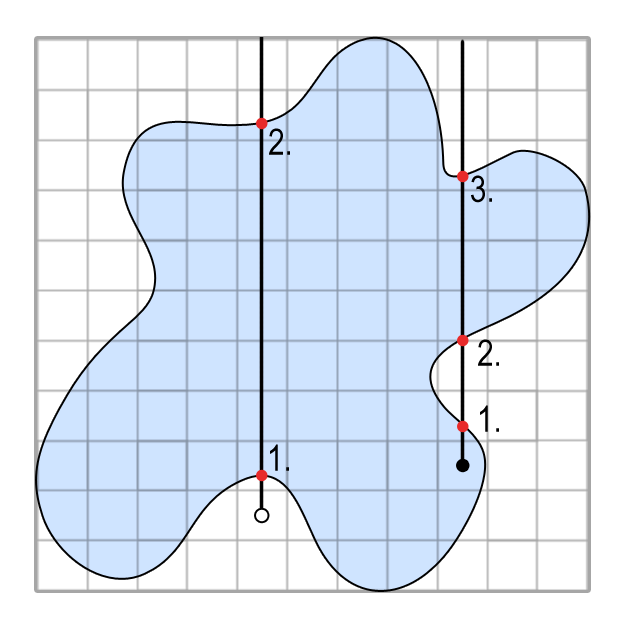
\includegraphics[width=0.6\textwidth]{ray.png}
	\caption{Vizualizácia algoritmu zisťovania, či sa bod náchádza v objekte}
	\label{ray}
\end{figure}


\subsubsection{Export}
Z každého voxelového objektu je možné extrahovať jeho povrchovú informáciu a vytvoriť z nej klasický 3D model.
Táto vlastnosť je užitočná napríklad pri postprocesingu, ak by sme napríklad chceli vytvoriť kvalitný render voxelových objektov.
Náš algoritmus prechádza všetky voxely v objekte, vypočíta pozíciu všetkých krajných 8 bodov voxelu a pre každý určí, či sa nachádza na povrchu objektu alebo nie. Následne tieto body pridá do poľa tak, aby sa v ňom nenachádzali duplicitne a do ďalšieho poľa si zapamätá poradie bodov, aby bolo možné danú viditeľnú stenu rekonštruovať.

\subsection{Bitmapa}
Do programu sme zahrnuli aj možnosť importovania bitmapy do prostredia. Spôsob, akým to robíme, je pomerne jednoduchý. Načítame si bitmapu zo súboru do pamäte a následne si vytvoríme voxelový objekt s hĺbkou 1 a šírkou a výškou rovnajúcimi sa rozmerom obrázka. Teraz nám stačí už len prejsť všetky body bitmapy a pridať voxel príslušnej farby do objektu. 

\subsection{Voxelové formáty}
Špecifikáciu bežne používaných voxelových formátov sme získali zo zdrojových kódov opensoruce programu \textit{binvox} \cite{binvox}. Vďaka tomu sa nám podarilo pridať do ponuky aplikácie pomerne veľké množstvo rôznych výstupných a vstupných formátov. 

\begin{multicols}{2}
Výstupné formáty:
\begin{itemize}
	\item Binvox
	\item RawVox
	\item Hips
	\item Mira
	\item Vt
	\item Vtk
\end{itemize}

Vstupné formáty:
\begin{itemize}
	\item Binvox
	\item Vox
	\item Mira
	\item Vt
	\item Vtk
\end{itemize}
\end{multicols}
Tieto formáty sa štruktúrou na seba dosť podobajú. Zaujímavým z nich je napríklad Binvox, ktorý používa RLE kódovanie na kompresiu dát a najjednoduchším z nich je RawVox, ktorý v sebe uchováva surové dáta tak, že na mieste voxelu ukladá $1$ a na mieste prázdneho miesta $0$.
Ich veľkou nevýhodou je, že nie je možné v nich ukladať viacej objektov naraz a taktiež neuchovávajú informáciu o farbe voxelov. Aby sme mohli ukladať celé scény pred začatím zapisovania dát do súboru, zlúčime všetky objekty v scéne a následne takto vzniknutý objekt uložíme.

\subsection{XML}
Keďže všetky známe formáty na ukladanie voxelov do súborov sú binárne a neumožňujú ukladanie farieb a ani celých scén s väčším množstvom objektov. Rozhodli sme sa ukladať scény do nami navrhnutej XML štruktúry. Takýto výstup je nielen viacej čitateľný, ale môžme si dovoliť uložiť akékoľvek informácie navyše, ktoré potrebujeme. Jeho nevýhodou oproti binárnym súborom je však jeho velkosť.
Import aj export XML sme implementovali prostredníctvom vyššie spomenutej knižnice \textit{pugixml}.
\eject
Takto vyzerá nami navrhnutá XML štruktúra:

\begin{framed}
\begin{lstlisting}
<?xml version="1.0" encoding="utf-8"?>
<cubo>
  <scene width="" height="" depth="">
    <positions>
      <position index="" x="" y="" z="" />
                    ...
    </positions>
    <objects>
      <object width="" height="" depth="" position="">
        <colors>
          <color index="" red="" green="" blue="" alpha="" />
                              ...
        </colors>
        <voxels sample="">
          <voxel i="" j="" k="" color="" />
                       ...
        </voxels>
      </object>
         ...
    </objects>
  </scene>
</cubo>
\end{lstlisting}

\end{framed}
